\chapter{Grafen}
	Zgodnie z najnowszą definicją grafen to: ,,Cienka monowarstwa zbudowana z atomów węgla,
ułożonych w dwywymiarowej sieci o stukturze plastra miodu. Grafen jest podstawowym budulcem
dla materiałów grafitowych o innych wymiarach. Może być zwinięty tworząc zerowymiarowe fullereny,
zrolowany w jednowymiarowe nanorurki lub spiętrzony w stos tworząc trójwymiarowy grafit''	
\footnote[1]{(odnośnik do Geim, A. K. and Novoselov, K. S. (2007). "The rise of graphene". Nature Materials 6 (3): 183–191. 					Bibcode:2007NatMa...6..183G. doi:10.1038/nmat1849. PMID 17330084.)}

	Ta definicja pokazuje, że grafen stanowił ważny materiał, zanim udało się znaleźć metodę jego otrzymywania, \footnote[2]{tutaj o początkach grafenu} ponieważ odgrywał ważną rolę w modelowaniu właściwości innych materiałów zbudowanych z węgla (fullereny, nanorurki).
	
Poniższy rozdział ma na celu przybliżenie własności grafenu, dzięki którym możliwe
zastosowania stanowią o niesamowitym zainteresowaniu ze strony dzisiejszych naukowców. Dodatkowo
zostanie zaprezentowana i omówiona metoda jego otrzymywania, w której upatruje się 
największe nadzieje na otrzymywanie przemysłowych ilości tego niezwykłego materiału.
Na sam koniec przedstawione zostaną niektóre z wielu zastosowań grafenu z naciskiem na
tranzystory polowe z kanałem grafenowym, które stanowią główną oś niniejszej pracy.

\newpage

	\section{Struktura atomowa i własności mechaniczne}
	Jeżeli skupimy się na pojedynczym atomie węgla tworzącym grafen, wtedy okaże się, że 
	mamy do czynienia z hybrydyzacją typu $\mathrm{sp^2}$. Takie oddziaływanie między
	orbitalami s i p prowadzi do powstania bardzo silnych wiązań typu $\sigma$ pomiędzy
	sąsiednimi atomami węgla. Te wiązania mają, zgodnie z zasadą Puliego, zapełnione 
	powłoki elektronowe i tworzą głębokie pasmo walencyjne. Długość tego wiązania wynosi
	1,42 Å i leżą one w jednej płaszczyźnie. To te wiązania decydują o tak dużej stabilności tego
	układu i o jego niezwykłych właściwościach mechanicznych. Wygląd tak powstałej sieci widoczny jest na 
	rysunku \ref{fig:siec_grafenu}. 
	
	\vspace{-10pt}
	\begin{figure}[ht]
	\centering
	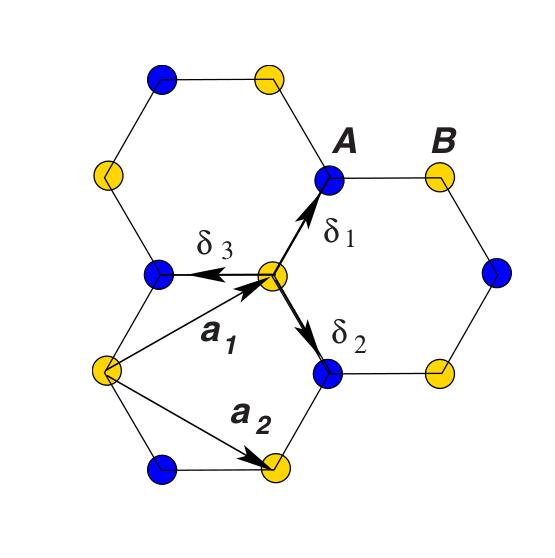
\includegraphics[width=0.50\textwidth]{./Rozdzial_2/obrazki/Siec_grafen.jpg}
	\caption{Sieć atomowa grafenu}
	\label{fig:siec_grafenu}
	\end{figure}
	\vspace{-10pt}

	Na rysunku możemy zobaczyć, że sieć grafenu zbudowana jest z dwóch dwuwymiarowych sieci Bravais'ego (kolory 
	niebieski i żółty), oznaczone literami A i B. Dodatkowo widoczne są wspomniane wcześniej trzy wiązania $\sigma$.
	Warto też wspomnieć o dwóch wektorach a$_1$ i a$_2$, tworzących pojedynczą sieć Bravais'ego. O ile nie mają one,
	większego znaczenia dla samego opisu grafenu, o tyle warto o nich wspomnieć w kontekście nanorurek węglowych. Dzięki
	wielokrotnościom tych wektorów określa się tak zwany wektor chiralności nanorurki. Dzięki temu można poznać charakter
	nanorurki (metaliczna czy półprzewodnikowa).
	
	Jako wynik takiej budowy sieci grafenu, jest on bardzo wytrzymały. Teoretycznie 100 razy bardziej wytrzymały niż
	stal o takiej samej grubości. Mimo wszystko jest on też bardzo lekki. Istnieje bardzo obrazowe
	porównanie obu tych właściwości. Gdyby wytworzyć grafenowy hamak o powierzchnii 1 m$^2$, to taki hamak byłby
	w stanie wytrzymać 4-kilogramowego kota. Jednocześnie sam hamak  ważyłby mniej niż jego pojedynczy wąs. 
	Dokładniej ważyłby 0.77 mg, jest to $10^{5}$ raza mniej niż waga arkusza papieru o tej samej powierzchni.

	\section{Struktura i własności elektroniczne}
	Po utworzeniu 3 par typu $\mathrm{sp^2}$ pozostaje jeden orbital typu p, będący prostopadły do
	powierzchni tworzonej przez wiązania typu $\sigma$. Wraz z niesparowanymi orbitalami typu p pochodzącymi od
	 sąsiednich atomów,  tworzy on zdelokalizowane wiązanie typu $\pi$
	Wiązania typu $\pi$ są znacznie słabsze niż wiązania typu $\sigma$. Dodatkowo są one 
	wypełnione tylko w połowie elektronami. Dlatego właśnie to wiązanie decyduje o niezwykłych właściwościach 
	elektronicznych grafenu.

	Na początku omówienia właściwości elektronicznych grafenu warto przedstawić sieć odwrotną dla tego materiału.
	Schemat pierwszej strefy Brillouina znajduje się na rysunku \ref{fig:siec_odwrotna}.
	
	\vspace{-10pt}
	\begin{figure}[ht]
	\centering
	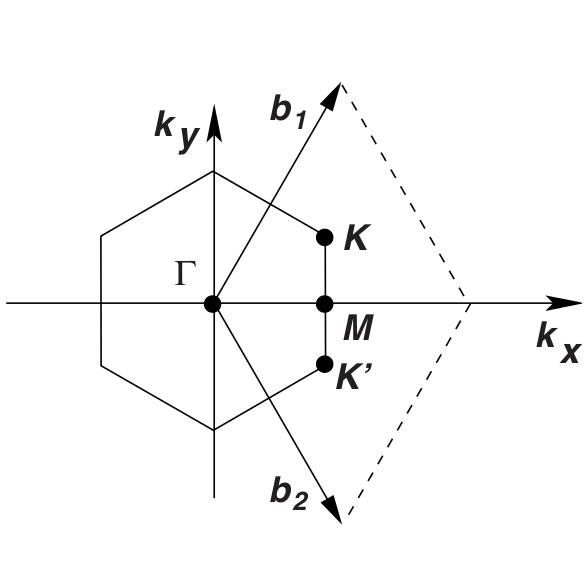
\includegraphics[width=0.50\textwidth]{./Rozdzial_2/obrazki/Siec_odwrotna.jpg}
	\caption{Sieć odwrotna grafenu}
	\label{fig:siec_odwrotna}
	\end{figure}
	\vspace{-10pt}
	Zaznaczone są na nim punkty wysokiej symetrii ($\Gamma$, K i M). Dodatkowo pokazane zostały wektory b$_1$ i b$_2$, 
	opisujące sieć odwrotną. Warto zauważyć, że sieć odwrotna bardzo przypomina sieć atomową. Z geometrycznego punktu
	widzenia sieć odwrotna jest to obraz sieci atomowej obrócony o 30$^o$. 
	Operując w sieci odwrotnej można wyprowadzić zależność energii od położenia na płaszczyźnie wektora k. Najprostszą
	metodą otrzymania takiej zależności jest metoda ciasnego wiązania (\textit{ang. Tight-binding method}). Prowadzi ona
	do następującej zależności energii:
	\begin{equation}
    		E(\vec k)_{\pm}=\pm t \sqrt{3+f(\vec k)} - t'f(\vec k)
		\label{equ:energia}
	\end{equation}
	\begin{equation}
    		f(\vec k)= 2\cos({\sqrt{3}k_y a}) + 4\cos \left (\frac{\sqrt{3}}{2} k_y a \right )\cos \left (\frac{3}{2}k_xa \right )
	\end{equation}

	Oznaczenie t występujące w zależności \ref{equ:energia} jest to energia przeskoku pomiędzy danym atomem a 
	jego najbliższym sąsiadem (zmiana podsieci). Natomiast t' jest to energia przeskoku pomiędzy następnym najbliższym
	sąsiadem. Wartość t$\approx$2,8 eV, natomiast t'$\approx$0,2 eV. Na podstawie oby tych zależności \ref{equ:energia}, został narysowany wykres zależności energii w pierwszej strefie Brillouina, który zostął przedstawiony na rysunku \ref{fig:Struktura_pasmowa}.Dodatkowo zaznaczony został obszar w pobliżu punktu K.

	\vspace{-10pt}
	\begin{figure}[ht]
	\centering
	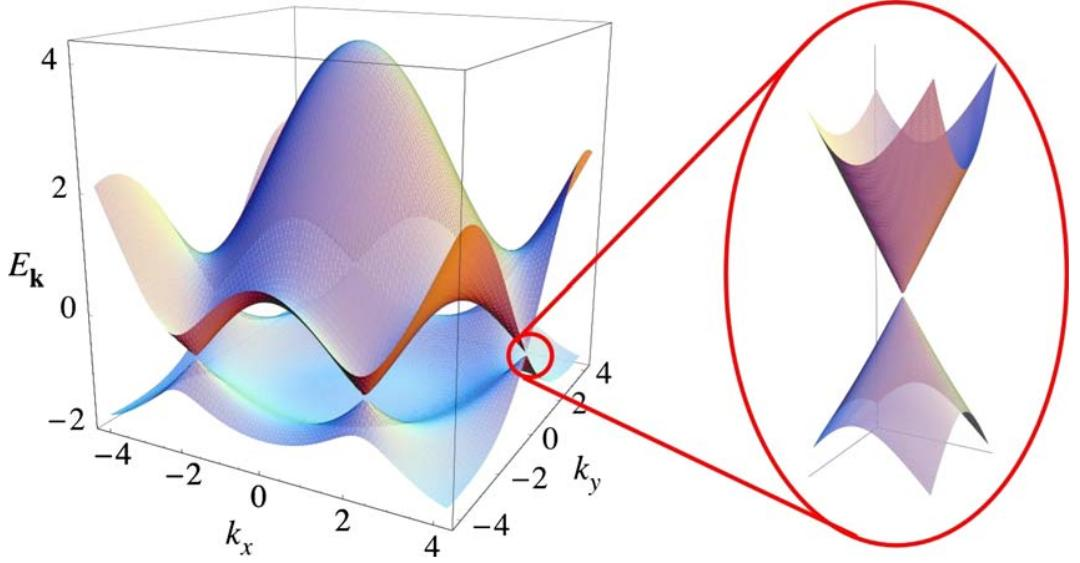
\includegraphics[width=0.80\textwidth]{./Rozdzial_2/obrazki/Struktura_pasmowa.jpg}
	\caption{Struktura pasmowa grafenu}
	\label{fig:Struktura_pasmowa}
	\end{figure}
	\vspace{-10pt}

	Wyróżniony obszar to tak zwany stożek Diraca. Jest to w zasadzie najciekawsze miejsce na krajobrazie pasmowym z 
	co najmniej dwóch powodów. Po pierwsze jest to miejsce, gdzie stykają się pasma przewodnictwa i walencyjne. 
	Po drugie w pobliżu punktu K mamy do czynienia z liniową zależnością energii od wektora falowego. 
	Najczęściej tą relację w przybliża się w następujący sposób:
	\begin{equation}
    		E(\vec k) = \pm v_F|\vec k|
	\end{equation}
	Gdzie $\vec k = \vec K + \vec q$ i jednocześnie $|\vec q| << |\vec K|$.

	\section{Grafen otrzymywany metodą CVD}
	Istnieje już dość duża liczba metod otrzymywania grafenu. Należy w tym miejscu wspomnieć chociażby o eksfoliacji
(tak zwana metoda noblowska) i o metodzie opartej na węgliku krzemu (SiC). Jednak najbardziej obiecującą metodą
wytwarzania grafenu na potrzeby przemysłu wydaje się być aktualnie metoda CVD (\textit{ang. Chemical Vapour Deposition}), czyli
metoda osadzania z gazów. Poniżej zostanie opisana w sposób ogólny ta technologia, dodatkowo zostaną przedstawione wyniki 
charakteryzacji grafenu otrzymanego tą metodą.
		\subsection{Opis metody}
		\subsection{Badania strukturalne grafenu}
	\section{Zastosowania}
